\documentclass[11pt]{article}
\usepackage[a4paper,compat2]{geometry}

\usepackage{natbib}
\bibliographystyle{apalike}

\usepackage{graphicx}

\usepackage{amsmath}
\newenvironment{example}{\par\smallskip\noindent\begingroup\small\textbf{\small Example\enskip}}{\endgroup\par\smallskip}

\begin{document}

\title{\bf Rstisim 1.0: Simulating the dynamics of sexually transmitted
infections in R}

\author{
\textbf{Christian L. Althaus} \\
Institute of Social and Preventive Medicine (ISPM)\\
University of Bern, Switzerland\\
\texttt{calthaus@ispm.unibe.ch}
\and 
\textbf{Janneke Heijne}\\
Institute of Social and Preventive Medicine (ISPM)\\
University of Bern, Switzerland\\
\texttt{jheijne@ispm.unibe.ch}
\and
\textbf{Adrian R\"ollin}\\
Department of Statistics and Applied Probability\\
National University of Singapore\\
\texttt{adrian.roellin@nus.edu.sg}
}

\date{}

\maketitle

\tableofcontents
\newpage

\section{Introduction}
Rstisim is an individual-based model to study the spread and transmission of sexually transmitted infections in a population. Mathematical modeling of infectious diseases has established itself as an important field to study the spread of diseases in animal and human populations \citep{Anderson:1991,Diekmann:2000,Keeling:2008}. More recently, individual-based models have come to attention as they allow to explicitly simulate the transmission of infections through sexual contacts between different individuals \citep{Kretzschmar:1996,Ghani:1997,Ploeg:1998,Turner:2006,Low:2007,Gray:2009,Leclerc:2009}. Rstisim has been developed with the aim to provide a novel, flexible model that can describe the transmission dynamics of any type of sexually transmitted infection in a given population. The model allows to assign different partnership formation processes that lead to a specific sexual network structure. Additional emphasis is put on disease progression in infected people, treatment seeking and partnership notification. Hence, the model is designed to evaluate the impact of different public health strategies. The Rstisim package is free and open-source and is released under GPL (General Public License).

In this manual, we describe some general concepts of the model in Section \ref{ch:concepts}. Section \ref{ch:install} shows how the software package can be installed and Rstisim can be run. A documentation of the user interface is given in Chapter \ref{ch:Rdocu}. Chapter \ref{ch:configuration} discusses the syntax of the configuration files which provide the parameters for the model. Chapter \ref{ch:examples} provides some examples on how to run and analyze simulations. An example of a configuration file that simulates the transmission dynamics of chlamydia in a UK population is given in the \emph{Appendix}.

\section{General concepts}
\label{ch:concepts}
The simulator is written in an object-oriented framework in C++ \citep{Stroustrup:2000}. To allow for a versatile user interface, it can be accessed as a library from the statistical software package R \citep{R:2008}. That is to say, the model can be run directly from R where model outpouts can be analyzed and converted into a graphical output (Figure \ref{fig:scheme}).

In the future, we will describe here the structure of the individual-based model itself. For the moment, we refer to \citet{Low:2007} as Rstisim is strongly influenced by the ClaSS model which is presented there.

\begin{figure}[h]
\begin{center}
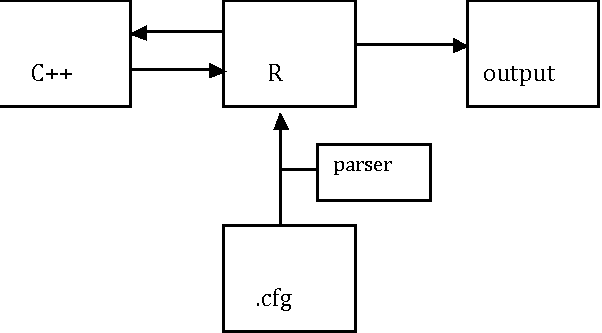
\includegraphics[width=8cm]{figures/scheme}
\end{center}
\caption{Scheme of the underlying structure of Rstisim. The statistical software package R reads in a configuration file (filename.cfg) through a parser. Once a simulation is started, R communicates with the simulator that is written in C++ to provide and access data. After a simulation run, graphical output can be directly generated from R.}
\label{fig:scheme}
\end{figure}

\section{Install and run Rstisim}
\label{ch:install}
\subsection{At the beginning}
% Rstisim can be installed and run on any system running Linux, Mac OS X or
% Windows. However, the system needs to have installed the statistical software
% package R. Optional packages are: latex (to create the documentation), dvipdf
% (dito), doxygen (for the C++ source code documentation) and gcc (GNU compiler
% collection to compile the source code into a library).

% First, one has to uncompress the package, get into the directory and run a
% script. This creates the Rstisim package, the R manual, the source code
% documentation and the stisim package. Under Linux, type:
% \begin{verbatim}
% $ tar xvzf stisim[version].tar.gz
% $ cd stisim
% $ ./create.sh
% \end{verbatim}
% 
% To build an R package, the stisim directory contains a subdirectory
% ``Rstisim'' with all the files needed to build an R package (the src directory
% contains links to the stisim/src directory). To build the package type (we
% assume that we are in the stisim directory), type
% \begin{verbatim}
% $ R CMD build Rstisim
% \end{verbatim}
% The above command builds a package named ``Rstisim[version].tar.gz'' in the
% current directory. 

To install the package in R under Linux, type
\begin{verbatim}
$ sudo R CMD INSTALL Rstisim_[version].tar.gz
\end{verbatim}
Under Windows or Mac OS X, use the graphical user interface to locate and
install the package.

Now you can run R, load the package and run simulations:
\begin{verbatim}
$ R
> library(Rstisim)
> sti.init("ex01.cfg")
> sti.run(365)
\end{verbatim}
The interface in R to run Rstisim is explained in more detail in Chapter \ref{ch:Rdocu}.

\subsection{Batch mode}
If one wants to run a long simulation run with a specified output, R allows to run Rstisim in batch mode. This is especially usefull if Rstisim is run on a remote machine via SSH:
\begin{verbatim}
ssh machine-name         # connect to a remote machine
R CMD BATCH run.R &      # start run in batch mode
exit                     # exit machine
\end{verbatim}
The file run.R can look like:
\begin{verbatim}
library(Rstisim)                 # load Rstisim package
sti.init("chlamydia.cfg")        # load configuration file
years<-10                        # the number of years the simulation should last
inf<-array(years)                # define an array to store data
for(i in 1:years) {              # loop to run the simulation
    sti.run(365)                 # for subsequent years
    inf[i]<-sti.infections()     # and store the data on infection in the array
}
q(save = "yes")                  # quit and save workspace
\end{verbatim}
The desired data is then store in the .RData file and can be accessed the next time the user invokes R in that directory.

Alternatively, one can append \texttt{R}-code to the configuration file using
the \verb|#EXECUTE| directive. This code will be automatically executed after
calling \verb|sti.init()| (see e.g.\ the example configuration
file \verb|ex06.cfg|).

\begin{verbatim}
#
# ... put the configuration of the model here
#

#EXECUTE

p = numeric(100)
for (i in 1:length(p)) {
  sti.run(365)
  p[i] = sti.prevalence(breaks=c(0,Inf))[[1]]
}
plot(p)
\end{verbatim}

This code will automatically run the simulation for 100 years and then plot the
prevalence in steps of one year.

\subsection{Error tracking}
To track down a segmentation fault, run R with a program like `valgrind':
\begin{verbatim}
> R -d "valgrind –leak-check=full"
\end{verbatim}
If you need to know the stack of the function calls and you know where the error
is produced, provoke a segmentation fault at that point on purpose. Insert
something like \texttt{((int *)0) = 1} and run software with valgrind.

\section{User interface in R}
\label{ch:Rdocu}
For the moment, we refer to the separate documentation ``Rstisim.pdf''.

\section{Configuration file}
\label{ch:configuration}

\subsection{Syntax}

\subsection{Distributions}

\subsubsection{Available distributions}

\paragraph{Constant distribution}
As everything in Rstisim is a distribution, so is (almost) every constant. Constants are specified by just giving the value directly: 
\begin{example}
\begin{verbatim}
 # every person lifes exactly 65 years
 lifespan = 65y;
 # every person that immigrates is of age 20 at the time of immigration
 immigrationage = 20y;
 # exactly every 10 days there is an immigration
 immigration = 10;
\end{verbatim}
\end{example}
Relative sampling is possible if the \emph{aleast}-value is below or equal to the specified one, otherwise an error is thrown (at run-time).

\paragraph{Discrete probability distribution}
This is a distribution that takes a finite set of values with certain probabilities. The simplest way to define such a distribution is through an array of length bigger than 1.
\begin{example}
\begin{verbatim}
 people = {
   names = ["male","female"];
   distribution = [.5, .5];
 }; 
\end{verbatim}
\end{example}
Here, the array \text{[.4, .6]} represents a distribution which takes the value 0 with probabilty $0.4$ and which takes the value 1 with probability $0.6$. So, if just an array is given, these values represent the probabilities of a
distribution on the numbers $0, 1, 2, 3, \dots$. If the numbers don't sum up to $1$, the array is normalized and a warning is given.

There is the potential for misspecification: \texttt{[1]} is interpreted as a constant and not as an array, so it represents the constant value 1 and not the value 0 with probability 1! Only if the array has at least length two the values are interpreted as probabilities.

If the distribution needs to take values other than $0, 1, 2, \dots$, discrete probability distributions can be defined by giving the \emph{values} that the distribution should take and the corresponding \emph{probabilities} as follows:
\begin{verbatim}
 { type="simple"; 
   [ probabilities=<array>; | survival=<array>; ]
   [ values=<array>; | from=<number>; [step=<number>;]] };
\end{verbatim}
If no \emph{values} are specified, the standard is to use $0,1,2,\dots$
depending on the length of the distribution, which must be defined in that case.
If \texttt{values} is specified, these are the values to be taken and the length
of that array must be equal to the length of the distribution. Alternatively one
can specify the values by using \texttt{from} and \texttt{step} (whose effect
is obvious). The default for step size is $1$. 

The distribution can be given either by the point probabilities or as a survival
function. If neither of the two is given a uniform distribution among the
values is constructed. If the probabilities don't sum up to 1, the
probabilities are standardised and a warning is given. The survival function
needs to be specified as in the following example:
\begin{verbatim}
 { type="simple"; survival=[1,0.8,0.3]; values=[0,1,2]; };
\end{verbatim}
The survival array needs to start with the value 1 (if not the array is divided
by this first number; this is convenient if the survival distribution is taken
from a lifetable which usually is normed to a fictive population size of
$100'000$). Thus, in the above example, the distribution takes the value $0$
with probability 0.2, the value 1 with probability 0.5 and the value 2 with the
remaining probability 0.3.

The form \texttt{\symbol{123} probabilities=[0.2, 0.1, 0.7];
\symbol{125};} is equivalent to just \texttt{[0.2, 0.1, 0.7];}. In both cases
the corresponding values that are taken are $0$, $1$ and $2$.

As this distribution is quite frequent, the \texttt{type="simple"} option can
be omitted in general or just be given by an array (as done in the
beginning of this section) which then fixes the possible values to $0$, $1$, $2$
up to the lenght-1 of the array.

\paragraph{Linearly interpolated distribution}

This distribution is defined through a density function, given at
a set of interpolation points.
\begin{verbatim}
 { type="linear";
   [ density=<array>; ] 
   [ values=<array>; | from=<number>; [step=<number>;]] };
\end{verbatim}
Outside of the specified values, the density is assumed to be zero. If
\texttt{density} is not specified, a constant density function is assumed,
resulting in a unifom distribution between the minimal and maximal values of
the given interpolation points. The given density function will be automatically
scaled so that it integrates to 1.

The \texttt{type="linear"} argument can be omitted if the \texttt{density}
argument is present. So do not forget to specify other distribution that also
have a \texttt{density} argument!

\textbf{Conditional sampling is currently not implemented and will produce an
error if requested!}

\paragraph{Uniform distribution}

This specifies a uniform distribution.
\begin{verbatim}
 { type="uniform"; [min = <number>;] [max = <number>;] };
\end{verbatim}
The minimum and maximum arguments are optional and, by default, set to $0$ and
$1$, respectively. While reading the configuration file, a uniform distribution
between $0$ and $1$ is added automatically to every part of the configuration
structure. This is done in order to sample events that happen with a certain
probabilty.

\paragraph{Simple exponential distribution}

This represents an exponential distribution (in contrast to the extended
version in the next paragraph). 
\begin{verbatim}
 { type="exponential"; [rate = <number>;] [shift = <number>;] };
\end{verbatim}
The shift is a number that is added to the exponential random number It is
fully integrated into the conditional sampling, ie.\ an exponential distribution
with shift 10 conditioned on being bigger than 3 is an exponential with shift
7. Accordingly, the same distribution conditioned on being bigger than 15 is
now a exponential without shift. 

If a rate argument is given, the \text{type="exponential";} argument can be
omitted.

Be careful when specifying the rate! The smaller the rate the less frequent the
events! So something like ``every 2 years'' has to be specified as
\texttt{\symbol{123} rate = 1/2y; \symbol{125};}
\begin{example}
\begin{verbatim}
 # On average, every day
 { rate = 1; };
 # On average every week
 { rate = 1/7; };
 # On average every year
 { rate = 1/1y; }; # Note that the "y" is binds stronger than the "/"
 # The same again
 { rate = 1/(1y); };
 # Again, on average every year
 { rate = 1/365; };
 # On average 365 times a day!
 { rate = 1y; }; # Usuallay not what is wanted
 # For the sake of completeness compare with contstant distribution:
 # Attention: the following is *not* half a year, its 1/730 of a day!!! 
 1/2y; 
 # You probably want
 0.5y; # or (1/2)y;
\end{verbatim}
\end{example}

\paragraph{Extended exponential distribution or inhomogenous Poisson
process}

The simple exponential distribution of the previous section allows only for
constant rate. If the rate of events should vary with the age of a
corresponding object (the rate at which a person initiates new partnerships
depends on its age), use the extended exponential distribution. So, this
distribution is usually only used in combination with \texttt{relativeto="age"}.
\begin{verbatim}
 { type="exponential"; relativeto="age"; density=<array>; 
   [ values=<array>; | from=<number>; [step=<number>;]]};
\end{verbatim}
The meaning of the arguments is very much the same as for the linearly
interpolated distribution. However, the so defined density function is
interpreted differenty, namely as the density of an inhomogeneous Poisson
process. If conditioned on being bigger than a certain value $x$, the distance
to the next point of the point process is returned. In areas with a higher
density functions, more events are likely to occur if the density is zero in an
area, no events will ever occurs there. This distribution will return the value
$\infty$ with a non-zero probability, as the support of the density is finite
and with a non-zero probabiltiy (namely with probabiliy $e^{-a}$, where $a$ is
the integral of the density function) the process will produce no points at
all, meaning that no finite next point exists. The value $\infty$ will be
interpreted by the simulation as \emph{never}, resulting in no future event
being installed. 

If the sampling from this distribution is done unconditional, this is as if
sampled conditioned on being at zero.

\paragraph{Extended constant distribution}

The constant distribution is not able to return values dependent on the age.
For this, the extended constant distribution is used. Again, this distribution
is only useful in combination with \texttt{relativeto="age"}.
\begin{verbatim}
 { type="constant"; relativeto="age"; density=<array>; 
   [ values=<array>; | from=<number>; [step=<number>;]]};
\end{verbatim}
The definition of the density is equivalend to the linearly interpolated and
the extended exponential distribution. 

The conditioning of this function is unlike conditioning of the other
distributions. Here, the conditioning value (the age of the object) is used as
the argument to the density function, ie.\ the value of the density function at
the location given by the age of the object is returned. So, for a given age,
the returned value is not random, but exactly specified by the density function.

\paragraph{Weibull distribution}

Use this distribution to sample from a Weibull distribution. 
\begin{verbatim}
 { type="weibull"; [shift = <number>;] 
   [scale = <number>;] [shape = <number>;] };
\end{verbatim}
The unshifted Weibull distribution is given by the cumulative distribution
function
\begin{equation}
 P[X\leq x] = 1-e^{-\left(\frac{x-\theta}{\lambda}\right)^\kappa},
	\qquad x\geq \theta,
\end{equation}
where $\lambda>0$ corresponds to the \texttt{scale} argument, $\kappa>0$
to the \texttt{shape} argument and $\theta$ to the \texttt{shift}
argument. Note that mean and variance of the shifted Weibull are 
\begin{equation}
\mathrm{E}(X) = \theta + \lambda\Gamma(1+1/\kappa), \qquad
\mathrm{Var}(X) = \lambda^2\left(\Gamma(1+2/\kappa)-\Gamma(1+1/\kappa)^2\right);
\end{equation}
see \texttt{http://en.wikipedia.org/wiki/Weibull\_distribution} for
more information about the Weibull distribution. Conditional sampling is not yet implemented for this distribution!

\subsubsection{Make distributions dependent on the state of objects}

This is a core concept of the Rstisim package and allows for great
flexibility in the behaviour of the model. Most sampling of random values of parameters in the simulation is done with
respect to an \emph{object} that can have an age (internally such an
object is called an \emph{ageable}), like a person, a partnership or an
infection (which object that is, is defined for each parameter, so see the
documentation about the parameters in the configuration file). Usually we want
make the time when events happen or the probabilties that certain events happen
dependent on the state of these objects, be that the age, the sex, the bin that
object is in. There are two distinct types of dependencies: age dependency and
dependency on countable properties that can be represented as non-negative
integers (e.g. the number of current partnerships of a person). 

Age dependency essentialy installes a single distribution that changes its
behaviour with the age of the object (age dependent rates at which something
happens depends). In contrast, dependecy on countable properties are constructed
through arrays of distributions and the distribution that is picked for sampling
is the one with the corresponding to the state of the property (no partnerships
corresponds to distribution at place 0, one partnhership to distribution 1, and
so on).

\paragraph{Age dependency and the \texttt{relativeto} option}

Age dependency is activated by using the \texttt{relativeto} option. Although
it can be used in principle for any distribution, its use is only meaningfull
in certain combinations.

Here are the available options:
\begin{itemize}
\item\textbf{Conditioned on age.} This can be activated by adding
\texttt{relativeto=``age''} to any distribution. In that case \emph{conditional
sampling} is used from the distribution, which in general means conditioned that
the returned value from the distribution is equal or bigger than the current age
of the underlying ageable object (the \emph{extended constant distribution}
being somewhat an exception; there the age is used more like a parameter). The
returned value is meant to be a value relative to the current time. 
\begin{example}
\begin{verbatim}
 # somewhere in the partnershipformer section
 seek =  { rate=1/1y; shift=12y; relativeto="age"; };
\end{verbatim}
In the above example the \texttt{seek} parameter is used to sample the
time point of the event that a person initiates a new partnership. The
distribution is an exponential distribution, shifted by 12 years. Now. the
following happens: at birth the first such event is sampled. In order to do
this, the above distribution is conditioned on being bigger than the age of
the person, which is 0, so the \texttt{relativeto} option has no effect at this
stage. However, assume that, 5 years later, we want to sample again such an
event in the future. Now, relative to now and conditioned on being bigger than 5
years, the above distribution has become an exponential distribution with the
same rate but now shifted only by 7 years (5 have passed already). What happens
7 years later? Now we end up with an unshifted exponential distribution. Now
increase the time again by, say, 5 years. So, the person is 17 years old. Now
we condition the above distribution on being atleast 17 years, and this is now
again an unshifted exponential distribution, as conditioning an exponential
distribution being bigger than, say, $x$, this is $x$ plus an exponential
distribution (this is called the \emph{lack of memory property} of the
exponential distribution).

What would happend without the  \texttt{relativeto="age"} statement? At birth
we would not notice a difference, but assume again 5 years passed and that we
now want to sample the next event. The distribtion would return an
unconditional sample that is a exponential plus 12 years, so the next event
would not take place before the object is 17y old, and every time we would
sample to get the new time point of the next event, we would get the additional
12 years. 
\end{example}

If the distribution is not evaluated with respect to an ageable (such as
sampling the immigration events) this feature has no effect. Usually this option
is used in combination with the distributions of type \emph{extended
exponential} and \emph{extended constant distributions}
\begin{example}(\texttt{visitgp} parameter of a person)  This parameter
regulates when people go to the GP irrespective of an infection. It
could be defined as
\begin{verbatim}
 visitgp = { type="exponential"; values=[12,35,65]y;
             density=[1/3y, 1/1y, 1/1y]; relativeto="age"; };
\end{verbatim}
In this form, each person of this type would go to the GP on average
every 3 years beginning at the age of 12, then going linearly up to (on average)
yearly visit at age 35, which then stays until 65, and after that drops down
to no visit to the GP. Without the keyword \texttt{relativeto} and if the time
point for a next testing event is to be sampled, it would return a value
somewhat bigger than 12 years, resulting in testing a bit more than every 12
years.
\end{example}

\item\textbf{Conditioned on the birth of the ageable.} Despite the naming,
actually \emph{unconditional} sampling is used if this option is activated by
adding \texttt{relativeto=``birth''} to any distribution. In that case
unconditional random sampling is used, but now the returend value is not added
to \emph{now} but to the time point of birth of the the underlying object. It
may thus happen that the resulting time point is a time point in the past. In
this case an error is thrown as it is not possible to insert events before the
current absolute time of the simulation. It is up to the user to make sure that
this does not happen.
\begin{example}
Let's look at the corresponding example as discussed in the paragraph about
conditioning on age:
\begin{verbatim}
 # somewhere in the partnershipformer section
 seek =  { rate=1/1y; shift=12y; relativeto="birth"; };
\end{verbatim}
Now, what happens? The distribution is always returning a (unconditional) sample
from an exponential distribution shifted by 12 years, but now relative to the
time of birth of the underlying object. The result seems the same as for
conditioning on the age. This is true until the age of 12 years. Assume than
the object is now 20 years old. The above distribution would now almost
certainly return a value in the past, as -20 years (the time of birth) plus 12
years plus an exponential of rate 1/1y is unlikely to be positive (which would
correspond to an event in the future).
\end{example}
So when is this feature needed, then? Consider the following example:
\begin{example} Assume
we have an infection that swiches between \emph{symptomatic} and
\emph{asymptomatic} states on average every week, but exactly a year after the
infection it is naturaly cleared (of course an unrealistic model, but let's
assume this for the sake of illustrating the feature). We could define the
\texttt{bin} section of an infection as
\begin{verbatim}
 bins = {
   names = ["asymptomatic","symptomatic","cleared","treated"];
   transitions = {
     # the names of the possible transitions
     names = ["a2s", "s2a", "a2c", "s2c"];
     # the definition of the transitions
     a2s = { from="asymptomatic"; to="symptomatic"; at={rate=1/7;}; };
     s2a = { from="asymptomatic"; to="symptomatic"; at={rate=1/7;}; };
     a2c = { from="asymptomatic"; to="cleared"; 
             at={values=1y; relativeto="birth"}; }; 
     s2c = { from="symptomatic"; to="cleared"; 
             at={values=1y; relativeto="birth"}; }; 
   };
 };
\end{verbatim}
Note that every infection always needs the two states \emph{cleared}
and \emph{treated}. In the above example we have to code the constant
distribution for the \texttt{at} parameter a bit more complicated than just
writing \texttt{at=1y;} because we want to activate the \texttt{relativeto}
option. So, \texttt{at=\symbol{123}values=1y;\symbol{125};} is also a
distribution with the constant value of 365 days where we can now add the
option if we like.

But let's first see what happens if we don't activate the \texttt{relativeto}
option. Sampling the next transition event is done by sampling the future time
point of every possible transition out of the current bin and then taking the
transition closest to now and discarding the other time points). So, if we would
specify the transition times into the \emph{cleared} state just by
\texttt{at=1y;} (or, as mentioned, by
\texttt{at=\symbol{123}values=1y;\symbol{125};}) and the infection is in the
\emph{asymptomatic} state the following happens. The simulation
samples the next transition by sampling from an exponential time with rate $1/7$
(that's the transition into the \emph{symptomatic} state) and also sample from
the constant distribution 365 (that's the transition into the \emph{cleared}
state). In that case, with probability almost one, the exponential time point is
smaller than the constant 365 and the infection would go into the
\emph{symptomatic} state (the probability that an exponential random variable
with rate 1/7 is bigger than 365 is $2.26\times10^{-23}$, so practically zero).
And this would now repeated the same way and the infection would switch between
the \emph{symptomatic} and \emph{asymptomatic} states almost \emph{ad 
infinitum}. So, that's not what we want. 

Specifying \texttt{at=\symbol{123}values=1y; relativeto="birth"\symbol{125};}
changes the behaviour. Now, the 365 days are with respect to the time of
infection (birth of the infection object). If we are 300 days after that time
the constant distribution would not return 365 but the difference relative to
the birth of the infection, so it would return 65. Coming closer to the time
point of 365 days after infection, the transition into the \emph{cleared} state
will eventually win the race against the exponential time.\footnote{Actually,
for a constant distribution as in this example, the \texttt{age} and
\texttt{birth} variants are equivalent, but this is true \emph{only} for the
constant distribution! An exponential distribution with
\texttt{relativeto="age"} will always return again an exponential time, because
an exponential time conditioned on being bigger than, say, $x$, has again an
exponential distribution (relative to $x$). However, an exponential distribution
with \texttt{relativeto="birth"} will return an exponential time minus the
current age of the object against which it is
evaluated, and this will eventually return a time point in the past,
producing an error.}
\end{example}

\item\textbf{Conditioned on absolute time.} This feature is sampling
conditioned on the acutal, absolute time. The simulation always starts at time
point $0$, so that with this feature parameter values can be changed as the
simulation runs. For example, to turn on background screening during years 50
to 60 of the simulation, the following can be used:
\begin{verbatim}
visitgp = { type="exponential"; relativeto="time";
values=[50,60]y; density=[1/1y, 1/1y]; };
\end{verbatim}

\item\textbf{Conditioned on the time of birth of the ageable.} Despite the
naming, actually \emph{unconditional} sampling is used if this option is
activated by adding \texttt{relativeto=``birth''} to any distribution. In that
case unconditional random sampling is used, but now the returend value is not
added to \emph{now} but to the time point of birth of the the underlying object.
It may thus happen that the resulting time point is a time point in the past. In
this case an error is thrown as it is not possible to insert events before the
current absolute time of the simulation. It is up to the user to make sure that
this does not happen.
\begin{example}
Let's look at the corresponding example as discussed in the paragraph about
conditioning on age:
\begin{verbatim}
# somewhere in the partnershipformer section
seek =  { rate=1/1y; shift=12y; relativeto="birth"; };
\end{verbatim}
Now, what happens? The distribution is always returning a (unconditional) sample
from an exponential distribution shifted by 12 years, but now relative to the
time of birth of the underlying object. The result seems the same as for
conditioning on the age. This is true until the age of 12 years. Assume than
the object is now 20 years old. The above distribution would now almost
certainly return a value in the past, as -20 years (the time of birth) plus 12
years plus an exponential of rate 1/1y is unlikely to be positive (which would
correspond to an event in the future).
\end{example}
So when is this feature needed, then? Consider the following example:
\begin{example} Assume
we have an infection that swiches between \emph{symptomatic} and
\emph{asymptomatic} states on average every week, but exactly a year after the
infection it is naturaly cleared (of course an unrealistic model, but let's
assume this for the sake of illustrating the feature). We could define the
\texttt{bin} section of an infection as
\begin{verbatim}
bins = {
  names = ["asymptomatic","symptomatic","cleared","treated"];
  transitions = {
    # the names of the possible transitions
    names = ["a2s", "s2a", "a2c", "s2c"];
    # the definition of the transitions
    a2s = { from="asymptomatic"; to="symptomatic"; at={rate=1/7;}; };
    s2a = { from="symptomatic"; to="asymptomatic"; at={rate=1/7;}; };
    a2c = { from="asymptomatic"; to="cleared"; 
    at={values=1y; relativeto="birth"}; }; 
    s2c = { from="symptomatic"; to="cleared"; 
    at={values=1y; relativeto="birth"}; }; 
  };
};
\end{verbatim}
Note that every infection always needs the two states \emph{cleared}
and \emph{treated}. In the above example we have to code the constant
distribution for the \texttt{at} parameter a bit more complicated than just
writing \texttt{at=1y;} because we want to activate the \texttt{relativeto}
option. So, \texttt{at=\symbol{123}values=1y;\symbol{125};} is also a
distribution with the constant value of 365 days where we can now add the
option if we like.

But let's first see what happens if we don't activate the \texttt{relativeto}
option. Sampling the next transition event is done by sampling the future time
point of every possible transition out of the current bin and then taking the
transition closest to now and discarding the other time points). So, if we would
specify the transition times into the \emph{cleared} state just by
\texttt{at=1y;} (or, as mentioned, by
\texttt{at=\symbol{123}values=1y;\symbol{125};}) and the infection is in the
\emph{asymptomatic} state the following happens. The simulation
samples the next transition by sampling from an exponential time with rate $1/7$
(that's the transition into the \emph{symptomatic} state) and also sample from
the constant distribution 365 (that's the transition into the \emph{cleared}
state). In that case, with probability almost one, the exponential time point is
smaller than the constant 365 and the infection would go into the
\emph{symptomatic} state (the probability that an exponential random variable
with rate 1/7 is bigger than 365 is $2.26\times10^{-23}$, so practically zero).
And this would now repeated the same way and the infection would switch between
the \emph{symptomatic} and \emph{asymptomatic} states almost \emph{ad 
infinitum}. So, that's not what we want. 

Specifying \texttt{at=\symbol{123}values=1y; relativeto="birth"\symbol{125};}
changes the behaviour. Now, the 365 days are with respect to the time of
infection (birth of the infection object). If we are 300 days after that time
the constant distribution would not return 365 but the difference relative to
the birth of the infection, so it would return 65. Coming closer to the time
point of 365 days after infection, the transition into the \emph{cleared} state
will eventually win the race against the exponential time.\footnote{Actually,
for a constant distribution as in this example, the \texttt{age} and
  \texttt{birth} variants are equivalent, but this is true \emph{only} for the
  constant distribution! An exponential distribution with
  \texttt{relativeto="age"} will always return again an exponential time,
because
  an exponential time conditioned on being bigger than, say, $x$, has again an
  exponential distribution (relative to $x$). However, an exponential
distribution
  with \texttt{relativeto="birth"} will return an exponential time minus the
  current age of the object against which it is
  evaluated, and this will eventually return a time point in the past,
  producing an error.}
  \end{example}
  
\item\textbf{No age dependency.} This is the default for any distribution if
the \texttt{relativeto} option is not used.
\end{itemize}

So, use the age dependency if you want to change the behaviour of a
distribution depending on the age of an object and use the birth dependency if
you want to have events happening at specific points in time of the life time of
an object. 

\paragraph{The  \texttt{depends} keyword and the array distribution}

A central feature of the Rstisim package is that distribution can be
chosen at run-time depending on various states of the underlying object, like
people, partnerships and infections. As mentioned, most distributions are
evaluated with respect to such an object and we have already seen how we can 
influence the distribution through the age of the object. 

To influence the distribution through countable properties, like the current
bin, the number of current partners, the pregnancy states of a female, the
\texttt{depends} keyword can be used. To illustrate how this feature works we
give an detailed example:
\begin{example} 
Let us have a look at an example for people initiating new partnerships. We
want to make this dependent on the number of current partners that the person
already has:
\begin{verbatim}
 seek = {
   depends = "currentpartners";
   0 : { rate = 1/1y; };
   1 : { rate = 1/3y; };
   5 : { rate = 0; };
 };
\end{verbatim}
This defines a distribution that consists of several other distributions, that
is, an array of distribution is created. The index of the array is given by the
attribute specified through the \texttt{depends} argument. In the above
example, a person with no partners initiates partnerships with a rate of one
new partnership per year. Once it has found a partner (either by initiating
it itself or by being found by others), the rate drops down to a rate
of one every three years. The gap between 1 and 5, that is the numbers 2, 3 and
4 are copied from the lower boundary of the gap, in our case 1 current
partner. If a person has 5 current partners it won't initiate new partnerships
anymore (but may well be found by others, that depends on the \texttt{accept}
argument). Look at the following variant: 
\begin{verbatim}
 seek = {
   depends = "currentpartners";
   0 : { rate = 1/1y; };
   1 : { rate = 1/3y; };
 };
\end{verbatim}
Here, the person will always initiate new partnerships, as again the lower
boundary is used for values within a gap, the gap here being 1 to infinity.
The one exception is a possible gap around 0. Here the upper boundary is used:
\begin{verbatim}
 seek = {
   depends = "currentpartners";
   5 : { rate = 1/3y; };
   6 : { rate = 1/10y; };
 };
\end{verbatim}
This tells the person to initiate new partnerships with a rate of 1 every 3
years if the person has up to 5 current partners, and, if more than 6, only with
a rate of 1 per 10 years. 
\end{example}

So, abstractly, an array distribution is defined by 
\begin{verbatim}
 { depends = <string>;
   [0 : <distribution>;]
   [1 : <distribution>;]
   [...]
   [k : <distribution>;]
   [...]
   [n : <distribution>;]
 };
\end{verbatim}
where \texttt{<distribution>} can be any other distribution or again an array
distribution. The number need not be goven in an ordered sequence but ordering
them certainly improves readability.

\begin{example}
\begin{verbatim}
 seek = {
   depends = "children";
   5 : { 
     depends = "currentpartners";
     0 : { rate = 1/1y; };
     1 : { rate = 1/3y; };
     2 : { rate = 0; };
   };
   6 : { rate = 0; };
 };
 accept = {
  depends = "children";
  7 : 1;
  8 : 0;
 };
\end{verbatim}
Here, as long as the person has no more than 5 children, a person will initiate
new partnerships according to the array distribution given by the array at 5.
If the person has 6 or more children, this person initiates no more
partnerships. However, the person will accept new partnerships with probability
1 if asked by other people up to 7 children, but if having 8 or more children,
the person would refuse new partnerships.
\end{example}

\newenvironment{wideitemize}{
    \begin{flushleft}\begin{list}{}
    {\renewcommand{\makelabel}{\entrylabel}
	\setlength{\itemsep}{0ex}
    \setlength{\labelwidth}{15em}
    \setlength{\leftmargin}{15.48em}
  }}%
{\end{list}\end{flushleft}}

In this way, array distributions can be arbitrarily nested. If an object does
not support a specific attribute it returns the value 0. The following
values for \texttt{depends} are supported in the current version: 
\begin{list}{}{\small
\renewcommand{\makelabel}{}
\setlength{\itemsep}{0ex}\labelwidth=11em\setlength{\leftmargin}{12em}}
\item[\tt currentpartners] the number of current partners,
\item[\tt totalpartners] the number of total partners the person had, including
the current ones,
\item[\tt withinpartners] the number of partners the person had in the last
period of time, given by the element \texttt{simulation.withintimelag} in the
configuration file.     
\item[\tt currentinfections] the number of current infections (does not include
those infections that are in either of the states \emph{cleared} or
\emph{treated};
\item[\tt totalinfections] the total number of infections this person ever had,
including the actual ones; 
\item[\tt withininfections] the number of infections the person had in the last
period of time, given by the element \texttt{simulation.withintimelag} in the
configuration file;
\item[\tt abortions] the number of abortions the person had;
\item[\tt pregnancies] the number of pregnancies the person had;
\item[\tt contacts] the total number of sexual contacts the person ever had;
\item[\tt unprotectedcontacts] the total number of unprotexted sexual contacts
the person ever had;
\item[\tt children] the number of children that the person produced (either as
mother or as father, if retraceable;
\item[\tt linknumber] the number of the link in a chain of partner
notifications. The index case gets linknumber 0, all its partners 1, the
partners of those 2 and so on. This feature is only allowed at specific places,
otherwise this number is not correctly set;
\item[\tt treatments] the number of treatments this person ever had;
\item[\tt ispregnant] the state of pregnancy; instead of numbers use `no'
(corresponding to 0) and `yes' (corresponding to 1); an object that cannot be
pregnant will thus always return `no';
\item[\tt isactive] whether the object is still active/alive or not; instead of
numbers use `no'
(corresponding to 0) and `yes' (corresponding to 1); for people, this should
always be `yes', as people removed from the population cannot be referenced; for
infections,  this is `yes' if it is in neither of the states `cleared' or 
`treated'; for partnerships, this is `yes' if the partnership is still on-going,
and
`no' if the partnership is broken up at the time of evaluating this feeture.
\item[\tt product] this evaluates all items and returns the product of these
values
\item[\tt sum] this evaluates all items and returns the sum

\item[\tt bin, type] see below
\item[\tt host] see below
\end{list}

\paragraph{The `bybin', `bytype' keywords}

A special and important case of array distributions are constructed by using
the type or the bin of an object. Here, instead of a number, the name of the
corresponding type or bin is given.\footnote{Internally, these names are
translated into numbers, ranging from 0 to the number of types or bins minus 1.
The order is the order given in the array where the type names or the bin names
are declared} Instead of \texttt{depends="bin";} and \texttt{depends="type";}
the shortcuts \texttt{bybin;} and \texttt{bytype;} can be used.
\begin{example}
\begin{verbatim}
 # at the beginning of the configuration file is the declaration of the person
 # types
 model : {
   population : {
     people = ["male", "female"];
   };
 };
 # [...]
 # in the partnership section
 accept = { bytype;
   male : 1; 
   female : { depends="ispregnant"; yes=0.5; no=0; };
 };
\end{verbatim}
In this example, people of type \emph{male} will accept a new partnership
with probability 1 and people of type \emph{female} with probabilty 0.5 if not
pregnant, but they would refuse if pregnant.
\end{example}

There is an important restriction to when the two keywords are allowed.
Depending on the context it may not make sense to set the \texttt{bytype}
option, as the type is already given. Look at the following exmple:
\begin{example}
\begin{verbatim}
 # somwhere in the section of the definition of an infection...
 immunity = { bybin; cleared = 1y; treated = 0.5y; * = 0; };
\end{verbatim}
The \texttt{immunity} argument defines the length of time that a person stays
immune after the infection was cleared naturally or after the infection was
treated. Note that, although this paramter is only used when the infection
enters either of these two states, we still need to give some values for all
other possible states (as the parser at the stage of parsing does not know the
meaning of the parameter and that the other states won't be used). Instead of
explicitely giving a value for each bin, we can provide a default value through
the \texttt{*} argument (this default value can be given for both,
\texttt{bytype} and \texttt{bybin}).
\end{example}

In this example, the \texttt{bytype} option would not make
sense because the parameter is evaluated with respect to the infection that is
defined in that very same section and not with respect of an arbitrary
infection. Let us look at another example:
\begin{example}
\begin{verbatim}
 # somewhere in the partnership section
 breakup = 1y;
 breakupfactorperson1 = {bytype; female=1; male=2;};
\end{verbatim}
First, note that \texttt{breakup} defines the time of the breakup and hence the
factor-feature is used for sampling (see Section~\ref{sssec:factor}), so that a
bigger value means a smaller time intervall. In the above configuration, every
partnership has a fixed base duration of 1 year; however, if the the first
person of the partnership (the initiator of the partnership if the `INDIVSEARCH'
partnership formator is used) is male, the duration is reduced to half a year. 
\end{example}
In the above example we must use the \texttt{bytype} option, because
\texttt{breakupfactorperson1} is a parameter evaluated with respect to the
first person in the partnership, and the section in which this parameter is
defined belongs to the section of partnerhship type. So, the underlying object
for this parameter is of a person type and
therefore we first have to specify the type of the person.
\begin{example}
\begin{verbatim}
 # somewhere in the partnership section
 breakup = 1y;
 breakupfactorperson1 = {bytype; female=1; male={bybin; core=3; noncore=1};};
\end{verbatim}
Again the base duration of each partnership is 1 year but now, if the first
person is a male and this male is in the bin \emph{core} the duration is
reduced to a third of a year. 
\end{example}


Summarizing, \texttt{bybin} is allowed only within a distribution where
the type is already specified, either from context or via \texttt{bytype}.
The \texttt{bytype} keyword can only be used for parameters
that are evaluated with respect to an object that is different from the one
where the parameter is defined.

\paragraph{The `host' keyword}

If the behaviour of infections is to be defined, one may want to make the
parameters depend on the host (for example on the sex or age of the host). For
this, the \texttt{host} option can be used, which switches the evaluation of a
parameter, that is evaluated with respect to the infection, to its host. Once
there, you can then use \texttt{bytype} and \texttt{bybin} to make the behaviour
depend on the state of the host.
\begin{example}
\begin{verbatim}
 # somwhere in the infection section
 immunity = {bybin; *=0;
   cleared : { host = {bytype; female=1y; male=2y;}; }; 
   treated : { 
     host = {
       type="constant"; relativeto="age"; 
       values=[0,50,100]y; density=[2,2,0]y; 
     }; 
   }; 
 };
\end{verbatim}
Let us see what this configuration does. Immunity is evaluated with respct to
the infection, if that infection enters one of the states \emph{cleared} or
\emph{treated}. If an infection is naturally cleared the immunity will last one
year in females and two years in males. If the infection is treated, however,
the duration of immunity will be independent of the sex of the host but depend
on the age of the host: up to an age of 50, the immunity will last two years,
but the drops down linearly until no immunity at the age of 100. Lets look at a
variant of the above example:
\begin{verbatim}
 # somwhere in the infection section
 immunity = {bybin; *=0;
   cleared : { host : { bytype; female=1y; male=2y; }; }; 
   treated : { 
     type="constant"; relativeto="age"; 
     values=[0,50,100]y; density=[2,2,0]y; 
   }; 
 };
\end{verbatim}
This is the same but without the \texttt{host} option if treated. What happens
now? The age is now the age of the infection, more precicely the age when the
infection enters one of the two immunity states. So, the immunity of the
host will last two years if the infection lasted no more than 50 years, and
then will go down to 0 if the duration of the infection approaches 100 years!
(not a very realistic assumption)! The following version is similar but with
more realistic values:
\begin{verbatim}
 # somwhere in the infection section
 immunity = {bybin; *=0;
   cleared : { host : { bytype; female=1y; male=2y; }; }; 
   treated : { 
     type="constant"; relativeto="age"; 
     values=[0,50,100y]; density=[0,2,2]y; 
   }; 
 };
\end{verbatim}
If cleared, we have the same situation as before. But if treated it depends on
the duration of infection when treated. If the infection is treated at an early
stage, the immunity will not last long. After 50 days of infection it reaches
the level of 2 years if immunity and this length of immunity is kept if the
infection lasted longer than 50 days; the last interpolation point of 100
years is just an extreme value that is unlikely to be reached by any infection.
So, what we simulate here is the assumption that if an infection is treated at
an early stage the host is not or hardly able to build up a good immune
response. 
\end{example}

% \subsubsection{Cores of random number generators}

\subsubsection{Sampling from distributions}

The bevaviour of most parts of the simulation is controled through
\emph{probability distributions}. Distributions are objects from which the
simulations samples values, be that the time of future events given as a certain
rate (e.g. the rate of seeking new partners) or probabilities that something
happens while something else is happening (e.g. probability of transmission of
an infection when a sexual contact happens). The flexibility of the software
comes from the fact that the user can (almost) freely choose from a set of
distributions and that these distribution can depend on various states of
certain objects (sex of person, age of infection, sex of the host, duration of
infection etc.). 

To understand how distributions are used in the simulation we need to go a
bit into the details. Every distribution has several ways in which random
numbers can be sampled from it. The basic four variants are:
\begin{enumerate}
\item\textbf{Simple random sampling}. This just returns a real random number
from the distribution. (Method~\texttt{dsample()}). \item\textbf{Integer-valued
simple random sampling}. This returns a random number from this distribution but
rounded to the next lower integer, i.e. \emph{floored}.
(Method~\texttt{isample()}). \item\textbf{Random sampling conditioned on being
atleast ${x}$}. This samples from the distribution conditional on being
at least $x$ (internally, the difference to $x$ is returned).
(Method~\texttt{dsample(double atleast)}).
\item\textbf{Integer-valued random sampling conditioned on being atleast $x$}.
This is the same as above but the value is floored.
(Method~\texttt{isample(double atleast)}).
\end{enumerate}

Using these four basic procedures, more complicated constructs are defined as
we are going to discuss in the following paragraphs. 

\paragraph{Sampling with an additional factor} \label{sssec:factor}

The sampling functions that return a real value allow for an additional factor.
In general this feature is used for scaling the time points of events. A lower
value of the factor results in an enlongation of the time, i.e.\ bigger time
intervals between events. Think of the factor as a factor to the rate that
something happens: the smaller the rate, the less frequent something happens and
thus the longer the time intervals are. It depends on the distribution what
exactly the effect of the factor is. 
\begin{example} (\texttt{seek}) This is the main distribution for the
partnership forming module that regulates when people initiate a new
partnership. In addition, \texttt{seekfactor} is used to scale this. Assume we
want people to form a new partnership on average every two years (independent
of their age, current number of parters, etc.) We could define:
\begin{verbatim}
 # initiate a new partnership on average every 2 years
 seek = { rate = 1/2y; };
 seekfactor = 1/2;
 accept = 1;
\end{verbatim}
The additional factor $1/2$ is necessary, because people initiate partnerships
and get targeted by people, who initiate a new partnership, so the overall
rate of new partnerships per person would be twice the \texttt{seek}-rate. By
scaling with $1/2$ we correct for this effect (of course, we could have just
defined the seek rate to \texttt{1/4y}, but with the factor things are a
bit clearer).
\end{example}

However, many parameters in the configuration file contain the part
`factor' in their name without making use of this feature. It often just means 
that the value of that parameter is just multiplied to
the value of some other parameter. This is usually the case when the value is
not meant to be a time interval. The exact use is explained in detail for every
parameter.
\begin{example} (\texttt{infectiousness} parameter of an
infection) 
This is the probability that a 
infection is transmitted if there is an unprotected sexual contact. In
addition, one can specify the optional parameter \texttt{infectiousnessfactor}.
This number is multiplied to the infectioness so that a smaller factor means
less infections. 
\end{example}

\paragraph{Sampling with respect to an ageable}

\paragraph{Factor and ageable combined}

In that case, first the factor is applied to the distribution, and then the age
of the ageable is used for relative sampling.

\paragraph{Which of the above methods will be used?}

Which of the above methods is used to sample from a specific
distribution depends on the context, is built-in and hence cannot be changed.
\begin{example}
\begin{verbatim}
 # somewhere in the person type section
 lifetime = { rate = 65y; };
\end{verbatim}
The \texttt{lifetime} defines the distribution that is used to sample the time
point of death of a person. As the person is just being created, it does not
make sense to sample with respect to this person.\footnote{One could think of
sampling with respect to the mother or the father of the person, so that maybe
children of a younger females have a different lifespan than of older females}

\begin{verbatim}
 # somewhere in the partnership section
 unprotected = { 
   type="constant"; relativeto="age";
   values=[0,1,100]y; density=[1,1,0];
 };
\end{verbatim}
This parameter is the probability that a sexual contact that happens is
unprotected. It is evaluated with respect to the partnership in which the
sexual contacts takes place. So, in the example above, this probability is
influenced by the age of the partnership. With the first year, all contacts are
unprotected and then it goes down to 0 until the partnership is 100 years old.
\end{example}

\section{Examples runs}
\label{ch:examples}
Here, we will provide some examples on how to run and analyze simulations in Rstisim.

\begin{thebibliography}{}

\bibitem[Anderson and May, 1991]{Anderson:1991}
Anderson, R.~M. and May, R.~M. (1991).
\newblock {\em {Infectious {D}iseases of {H}umans: {D}ynamics and {C}ontrol}}.
\newblock Oxford University Press, Oxford.

\bibitem[Diekmann and Heesterbeek, 2000]{Diekmann:2000}
Diekmann, O. and Heesterbeek, J. A.~P. (2000).
\newblock {\em {Mathematical {E}pidemiology of {I}nfectious {D}iseases: {M}odel
{B}uilding, {A}nalysis, and {I}nterpretation}}.
\newblock John Wiley, Chichester.

\bibitem[Ghani et~al., 1997]{Ghani:1997}
Ghani, A.~C., Swinton, J., and Garnett, G.~P. (1997).
\newblock {The role of sexual partnership networks in the epidemiology of
gonorrhea}.
\newblock {\em Sex Transm Dis}, 24(1):45--56.

\bibitem[Gray et~al., 2009]{Gray:2009}
Gray, R.~T., Beagley, K.~W., Timms, P., and Wilson, D.~P. (2009).
\newblock {Modeling the Impact of Potential Vaccines on Epidemics of Sexually
Transmitted {C}hlamydia trachomatis Infection}.
\newblock {\em J Infect Dis}, 199(11):1680--1688.

\bibitem[Keeling and Rohani, 2008]{Keeling:2008}
Keeling, M.~J. and Rohani, P. (2008).
\newblock {\em {Modeling {I}nfectious {D}iseases in {H}umans and {A}nimals}}.
\newblock Princeton University Press, Princeton.

\bibitem[Kretzschmar et~al., 1996]{Kretzschmar:1996}
Kretzschmar, M., van Duynhoven, Y.~T., and Severijnen, A.~J. (1996).
\newblock {Modeling prevention strategies for gonorrhea and Chlamydia using
stochastic network simulations}.
\newblock {\em Am J Epidemiol}, 144(3):306--317.

\bibitem[Leclerc et~al., 2009]{Leclerc:2009}
Leclerc, P.~M., Matthews, A.~P., and Garenne, M.~L. (2009).
\newblock {Fitting the HIV epidemic in Zambia: a two-sex micro-simulation
model}.
\newblock {\em PLoS One}, 4(5):e5439.

\bibitem[Low et~al., 2007]{Low:2007}
Low, N., McCarthy, A., Macleod, J., Salisbury, C., Campbell, R., Roberts,
T.~E., Horner, P., Skidmore, S., Sterne, J. A.~C., Sanford, E., Ibrahim, F.,
Holloway, A., Patel, R., Barton, P.~M., Robinson, S.~M., Mills, N., Graham,
A., Herring, A., Caul, E.~O., Davey~Smith, G., Hobbs, F. D.~R., Ross, J.
D.~C., and Egger, M. (2007).
\newblock {Epidemiological, social, diagnostic and economic evaluation of
population screening for genital chlamydial infection}.
\newblock {\em Health Technol Assess}, 11(8):iii--iv, ix--xii, 1--165.

\bibitem[Stroustrup, 2000]{Stroustrup:2000}
Stroustrup, B. (2000).
\newblock {\em {The C++ Programming Language}}.
\newblock Addison-Wesley Longman Publishing Co., Inc., Boston, MA, USA.

\bibitem[Turner et~al., 2006]{Turner:2006}
Turner, K. M.~E., Adams, E.~J., Gay, N., Ghani, A.~C., Mercer, C., and Edmunds,
W.~J. (2006).
\newblock {Developing a realistic sexual network model of chlamydia
transmission in {Britain}}.
\newblock {\em Theor Biol Med Model}, 3:3.

\bibitem[Van~der Ploeg et~al., 1998]{Ploeg:1998}
Van~der Ploeg, C. P.~B., Van~Vliet, C., De~Vlas, S.~J., Ndinya-Achola, J.~O.,
Fransen, L., Van~Oortmarssen, G.~J., and Habbema, J. D.~F. (1998).
\newblock {{STDSIM}: A Microsimulation Model for Decision Support in {STD}
Control}.
\newblock {\em Interfaces}, 28(3):84--100.

\end{thebibliography}

\end{document}

